\documentclass[12pt,a4paper]{article}

%--- Packages ---
\usepackage[margin=2.5cm, headheight=15pt]{geometry}
\usepackage{titlesec}
\usepackage{xcolor}
\usepackage{mdframed}
\usepackage{booktabs}
\usepackage{array}
\usepackage{tabularx}
\usepackage{amsmath}
\usepackage{amssymb}
\usepackage{enumitem}
\usepackage{hyperref}
\usepackage{fancyhdr}
\usepackage{tcolorbox}
\usepackage{parskip}
\usepackage{graphicx}
\usepackage{float}
\usepackage{caption}
\usepackage{subcaption}
\usepackage{listings}
\usepackage{algorithm}
\usepackage{algpseudocode}
\usepackage{multicol}
\usepackage{cite}
\usepackage{tikz}
\usetikzlibrary{arrows.meta, positioning, shapes.geometric}

%--- Colors ---
\definecolor{primaryblue}{RGB}{5,50,115}
\definecolor{accentteal}{RGB}{0,110,100}
\definecolor{accentorange}{RGB}{190,75,10}
\definecolor{accentred}{RGB}{160,20,20}
\definecolor{accentgreen}{RGB}{20,130,60}
\definecolor{lightblue}{RGB}{215,230,255}
\definecolor{lightyellow}{RGB}{255,252,215}
\definecolor{lightgreen}{RGB}{215,245,215}
\definecolor{lightred}{RGB}{255,225,225}
\definecolor{codebg}{RGB}{245,245,248}
\definecolor{darkgray}{RGB}{55,55,55}
\definecolor{midgray}{RGB}{110,110,110}

%--- Hyperref ---
\hypersetup{colorlinks=true,linkcolor=primaryblue,urlcolor=accentteal,
  citecolor=accentteal,pdftitle={EN2150 A04 SC-OSPF Report}}

%--- Section Formatting ---
\titleformat{\section}{\color{primaryblue}\Large\bfseries}{\thesection}{1em}{}[\color{primaryblue}\titlerule]
\titleformat{\subsection}{\color{accentteal}\large\bfseries}{\thesubsection}{1em}{}
\titleformat{\subsubsection}{\color{accentorange}\normalsize\bfseries}{\thesubsubsection}{1em}{}

%--- Header/Footer ---
\pagestyle{fancy}\fancyhf{}
\fancyhead[L]{\color{primaryblue}\small EN2150 -- Communication Network Engineering}
\fancyhead[R]{\color{primaryblue}\small Assignment 04 -- SC-OSPF Protocol Design}
\fancyfoot[C]{\color{darkgray}\thepage}
\renewcommand{\headrulewidth}{0.4pt}

%--- tcolorboxes ---
\tcbuselibrary{skins,breakable}
\newtcolorbox{keybox}[1][]{colback=lightblue,colframe=primaryblue,coltitle=white,fonttitle=\bfseries,title=#1,breakable}
\newtcolorbox{designbox}[1][]{colback=lightgreen,colframe=accentteal,coltitle=white,fonttitle=\bfseries,title=#1,breakable}
\newtcolorbox{warningbox}[1][]{colback=lightred,colframe=accentred,coltitle=white,fonttitle=\bfseries,title=#1,breakable}
\newtcolorbox{notebox}[1][]{colback=lightyellow,colframe=orange!75!black,coltitle=white,fonttitle=\bfseries,title=#1,breakable}

%--- Listings (code style) ---
\lstset{
  backgroundcolor=\color{codebg},
  basicstyle=\ttfamily\footnotesize,
  breaklines=true,
  frame=single,
  framerule=0.5pt,
  rulecolor=\color{primaryblue!50},
  numbers=left,
  numberstyle=\tiny\color{midgray},
  keywordstyle=\color{primaryblue}\bfseries,
  commentstyle=\color{accentteal}\itshape,
  stringstyle=\color{accentorange},
  showstringspaces=false,
  tabsize=4,
  captionpos=b
}

%--- Caption style ---
\captionsetup{font=small,labelfont={bf,color=primaryblue},
  format=hang,justification=centering}

\begin{document}

%=========================================================
%  TITLE PAGE
%=========================================================
\begin{titlepage}
\centering
% \includegraphics[width=3cm]{logo.pdf}% Upload a logo to Overleaf and place its filename here
% fallback if logo not found — just skip it
\vspace*{0.5cm}

{\color{primaryblue}\rule{\textwidth}{1.5pt}}\\[0.5cm]
{\color{primaryblue}\Huge\bfseries SC-OSPF: Secure \& Centralized OSPF}\\[0.3cm]
{\color{primaryblue}\Large\bfseries A Novel Routing Protocol Design}\\[0.3cm]
{\color{accentteal}\large EN2150 -- Communication Network Engineering}\\[0.2cm]
{\color{darkgray}\large Assignment 04 -- Routing Protocol Design}\\[0.5cm]
{\color{primaryblue}\rule{\textwidth}{1.5pt}}\\[1cm]

\begin{mdframed}[backgroundcolor=lightblue,linecolor=primaryblue]
\centering
{\color{primaryblue}\large\bfseries Group Members}\\[0.5cm]
\begin{tabular}{ll}
\toprule
\textbf{Name} & \textbf{Index Number} \\
\midrule
Heshan Ranasinghe & 230521E \\
Heshan Ranasinghe & 230521E \\
Heshan Ranasinghe & 230521E \\
Heshan Ranasinghe & 230521E \\
\bottomrule
\end{tabular}
\end{mdframed}

\vspace{0.8cm}
{\color{darkgray}\large
  Department of Electronic \& Telecommunication Engineering\\[0.2cm]
  University of Moratuwa\\[0.2cm]
  Semester 4, Batch 23\\[0.2cm]
  \today
}\\[1.2cm]

\begin{mdframed}[backgroundcolor=lightgreen,linecolor=accentteal]
\textbf{\color{accentteal}Abstract}\\[4pt]
This report presents SC-OSPF (Secure \& Centralized OSPF), a novel routing
protocol that addresses two critical limitations of standard OSPF: the absence
of strong Link State Advertisement (LSA) authentication and inefficient
flooding-based convergence. SC-OSPF introduces HMAC-SHA256 cryptographic
signing for all LSAs and replaces distributed flooding with a centralized
controller model inspired by Software Defined Networking (SDN). Simulation
results using Python and NetworkX demonstrate that SC-OSPF achieves convergence
in a constant 2 rounds regardless of network size, compared to OSPF's
diameter-dependent growth, while reducing control message overhead by up to 98\%.
The proposed protocol completely blocks LSA injection attacks that corrupt 100\%
of routing tables in standard OSPF.
\end{mdframed}
\end{titlepage}

%--- Table of Contents ---
\tableofcontents\newpage

%=========================================================
\section{Introduction}
%=========================================================

The internet is built upon a foundation of routing protocols that enable packets
to traverse complex networks of interconnected routers. These protocols determine
the paths data takes across the network and form the critical control
infrastructure upon which all communication depends. Among the most widely
deployed intra-domain routing protocols is OSPF (Open Shortest Path First), a
link-state protocol defined in RFC~2328~\cite{rfc2328} that is deployed in the
majority of enterprise and service provider networks today.

Despite its widespread adoption, OSPF has significant limitations that have
become increasingly problematic as network scale, complexity, and security
requirements have grown. This assignment addresses two of the most critical
deficiencies:

\begin{enumerate}[itemsep=4pt]
  \item \textbf{Security}: Standard OSPF lacks mandatory strong authentication
  for Link State Advertisements (LSAs). A compromised or malicious router can
  inject forged LSAs, corrupting the Link State Database (LSDB) of all routers
  in the domain and causing traffic misdirection or denial of service.

  \item \textbf{Convergence Efficiency}: OSPF relies on wave-by-wave LSA
  flooding, where convergence time grows with the network diameter. In large
  networks, this results in stale routing tables and packet loss during
  topology changes.
\end{enumerate}

To address these limitations, this report proposes \textbf{SC-OSPF} (Secure \&
Centralized OSPF), a novel routing protocol that integrates HMAC-SHA256
cryptographic authentication with a Software Defined Networking (SDN)-inspired
centralized controller architecture. The protocol is designed to be deployable
in enterprise and campus networks as a drop-in improvement over standard OSPF,
with a graceful fallback mechanism should the controller become unavailable.

The remainder of this report is organized as follows: Section~2 reviews existing
routing protocols and their limitations. Section~3 presents the SC-OSPF protocol
design in full technical detail. Section~4 analyzes performance results from
simulation. Section~5 evaluates security and scalability. Section~6 presents the
simulation setup. Section~7 concludes the report.

%=========================================================
\section{Existing Protocols and Their Limitations}
%=========================================================

\subsection{RIP -- Routing Information Protocol}

RIP~\cite{rfc1058,rfc2453} is a distance-vector protocol in which each router
maintains a table of (destination, cost, next-hop) entries and shares its
complete distance vector with directly connected neighbors every 30 seconds.
The metric used is hop count.

\begin{warningbox}[Key Limitations of RIP]
\begin{itemize}[itemsep=4pt]
  \item \textbf{Count-to-Infinity}: When a link fails, routers may continuously
  increment the metric toward infinity before declaring a destination
  unreachable. RIP defines infinity as 16 hops, making recovery extremely slow
  (potentially 16 update cycles $\times$ 30 seconds = 8 minutes).

  \item \textbf{Maximum Network Diameter}: The 16-hop limit makes RIP unsuitable
  for large networks. Any destination more than 15 hops away is considered
  unreachable.

  \item \textbf{No CIDR Support (RIPv1)}: RIPv1 does not carry subnet mask
  information, making it incompatible with modern CIDR-based addressing.

  \item \textbf{No Security}: RIP messages are sent in plaintext. Any on-path
  attacker can inject false distance vectors, causing traffic misdirection.

  \item \textbf{Poor Convergence}: The 30-second periodic update timer means
  topology changes can take minutes to propagate across the network.
\end{itemize}
\end{warningbox}

\subsection{OSPF -- Open Shortest Path First}

OSPF~\cite{rfc2328,rfc5340} is a link-state protocol. Each router floods a
Link State Advertisement (LSA) describing its directly connected links to all
other routers in the area. Once every router has received all LSAs, it builds a
complete topology map (the LSDB) and independently runs Dijkstra's shortest path
algorithm to compute routing tables.

\begin{warningbox}[Key Limitations of OSPF]
\begin{itemize}[itemsep=4pt]
  \item \textbf{Weak or Absent Authentication}: RFC~2328 defines three
  authentication modes: None (Type 0), Simple Plaintext Password (Type 1), and
  Cryptographic MD5 (Type 2). Authentication is optional and disabled by default
  in many deployments. MD5, while better than nothing, is considered
  cryptographically weak by modern standards. A router with no authentication
  will accept any LSA, regardless of its true origin.

  \item \textbf{LSA Injection Vulnerability}: Without strong authentication, an
  adversary who gains access to any router (or the network segment) can craft
  fake LSAs with arbitrary link costs, impersonating legitimate routers. This
  causes all other routers to compute incorrect paths, enabling traffic
  interception or blackholing.

  \item \textbf{Flooding Overhead and Convergence Time}: LSA flooding propagates
  in waves outward from the originating router. In a network with diameter $D$
  (the longest shortest path), convergence requires $D$ flooding rounds. Each
  round involves $O(N \cdot E)$ messages in total, where $N$ is the number of
  routers and $E$ is the number of links. As measured in our simulation, a
  50-router network requires 7 flooding rounds and 9,800 control messages.

  \item \textbf{Per-Router Dijkstra Overhead}: Every router independently runs
  Dijkstra's algorithm ($O(N^2)$ or $O((N+E)\log N)$ with a priority queue)
  when convergence occurs. In large networks, this CPU overhead degrades
  forwarding performance.

  \item \textbf{LSDB Synchronization}: After a partition and reconnection, OSPF
  must re-synchronize full LSDBs between previously separated areas, causing
  significant transient overhead.
\end{itemize}
\end{warningbox}

\subsection{IS-IS -- Intermediate System to Intermediate System}

IS-IS~\cite{rfc1142,rfc1195} is another link-state protocol, functionally
similar to OSPF but defined by ISO rather than IETF. It is widely used in
large ISP backbone networks due to its scalability and vendor support.

\begin{warningbox}[Key Limitations of IS-IS]
\begin{itemize}[itemsep=4pt]
  \item \textbf{No Native Authentication by Default}: IS-IS TLV (Type-Length-Value)
  authentication exists but is not mandatory. Many deployments run IS-IS without
  authentication, exposing them to the same LSP injection attacks as unauthenticated OSPF.

  \item \textbf{Complex TLV Architecture}: IS-IS uses a highly extensible but
  complex TLV encoding. Vendor-specific TLVs create interoperability issues
  between different equipment manufacturers.

  \item \textbf{Flooding Convergence Limitation}: Like OSPF, IS-IS relies on
  flooding to distribute Link State Packets (LSPs). Convergence time scales with
  network diameter and is sensitive to flood timer settings.

  \item \textbf{Metric Limitations}: The original IS-IS specification defines a
  maximum metric value of 1023 per link and 16383 end-to-end. While extended
  metrics (up to $2^{24}-2$) were introduced later \cite{fortz2002}, not all
  implementations support them, limiting traffic engineering capabilities.
\end{itemize}
\end{warningbox}

\subsection{BGP -- Border Gateway Protocol}

BGP~\cite{rfc4271} is the inter-domain routing protocol of the internet. It is
a path-vector protocol used between Autonomous Systems (ASes) to exchange
reachability information and enforce routing policy.

\begin{warningbox}[Key Limitations of BGP]
\begin{itemize}[itemsep=4pt]
  \item \textbf{Extremely Slow Convergence}: BGP convergence after a topology
  change can take from seconds to several minutes. The Minimum Route
  Advertisement Interval (MRAI, typically 30 seconds for eBGP) deliberately
  throttles update frequency, introducing long periods of stale routing state.

  \item \textbf{Route Hijacking}: Because BGP originally had no authentication
  mechanism, any AS could announce prefixes it does not own. The famous 2008
  Pakistan Telecom incident caused YouTube to become globally unreachable for
  approximately two hours due to an erroneous BGP hijack. RPKI (Resource Public
  Key Infrastructure) was introduced to mitigate this but is not universally
  deployed.

  \item \textbf{No Strong Authentication}: BGP sessions use TCP MD5 signatures
  (RFC~2385) for session authentication, but route content itself is not
  cryptographically verified. BGPsec (RFC~8205) adds path authentication but
  has very limited deployment.

  \item \textbf{Policy Complexity}: BGP route selection involves up to 14
  decision steps, and misconfiguration is extremely common. Policy errors can
  propagate globally before being detected.
\end{itemize}
\end{warningbox}

\subsection{Comparative Summary}

\begin{center}
\begin{tabular}{lcccc}
\toprule
\textbf{Limitation} & \textbf{RIP} & \textbf{OSPF} & \textbf{IS-IS} & \textbf{BGP} \\
\midrule
No strong authentication    & \color{accentred}$\bullet$ & \color{accentred}$\bullet$ & \color{accentred}$\bullet$ & \color{accentred}$\bullet$ \\
Slow convergence            & \color{accentred}$\bullet$ & \color{accentred}$\bullet$ & \color{accentred}$\bullet$ & \color{accentred}$\bullet$ \\
Count-to-infinity           & \color{accentred}$\bullet$ & \color{accentgreen}$\circ$ & \color{accentgreen}$\circ$ & \color{accentgreen}$\circ$ \\
Network size limitation     & \color{accentred}$\bullet$ & \color{accentgreen}$\circ$ & \color{accentgreen}$\circ$ & \color{accentgreen}$\circ$ \\
LSA/LSP injection risk      & \color{accentred}$\bullet$ & \color{accentred}$\bullet$ & \color{accentred}$\bullet$ & \color{accentred}$\bullet$ \\
Flooding overhead           & \color{accentgreen}$\circ$ & \color{accentred}$\bullet$ & \color{accentred}$\bullet$ & \color{accentgreen}$\circ$ \\
Policy complexity           & \color{accentgreen}$\circ$ & \color{accentgreen}$\circ$ & \color{accentgreen}$\circ$ & \color{accentred}$\bullet$ \\
\bottomrule
\multicolumn{5}{l}{\footnotesize $\bullet$ = affected, $\circ$ = not significantly affected}
\end{tabular}
\end{center}

SC-OSPF specifically targets OSPF's \textbf{authentication} and \textbf{convergence
overhead} weaknesses as its primary focus, while the design principles are
applicable to IS-IS as well.

%=========================================================
\section{Proposed Protocol: SC-OSPF}
%=========================================================

\subsection{Design Philosophy}

SC-OSPF is designed around two guiding principles drawn from modern network
engineering:

\begin{enumerate}[itemsep=5pt]
  \item \textbf{Security by Construction}: Rather than bolting authentication
  onto an existing protocol as an afterthought, SC-OSPF requires every LSA to be
  cryptographically signed using HMAC-SHA256 before the controller will process
  it. An unsigned or incorrectly signed LSA is silently discarded. There is no
  ``unauthenticated'' mode.

  \item \textbf{Centralized Control, Distributed Forwarding}: Inspired by SDN
  (as studied in Session 6 of EN2150), SC-OSPF moves the control plane
  (topology collection and route computation) to a central controller while
  keeping the data plane (packet forwarding) at each individual router. This
  eliminates wave-by-wave flooding and enables constant-time convergence.
\end{enumerate}

\subsection{System Architecture}

\begin{figure}[H]
\centering
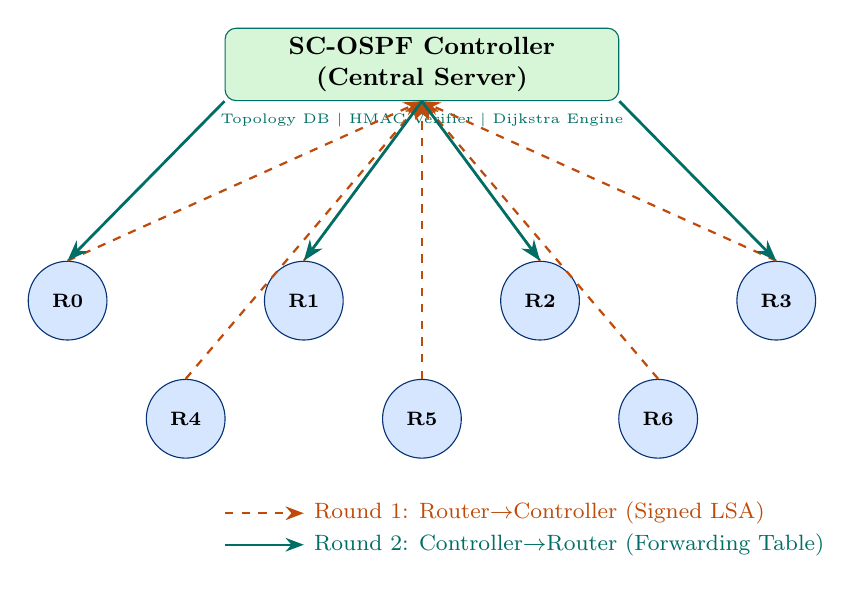
\begin{tikzpicture}[
  box/.style={draw,rounded corners=4pt,minimum width=2.8cm,minimum height=0.9cm,
              font=\small\bfseries,align=center},
  router/.style={draw,circle,minimum size=1cm,font=\scriptsize\bfseries,
                 fill=lightblue,draw=primaryblue},
  arr/.style={-{Stealth},thick}
]

% Controller
\node[box,fill=lightgreen,draw=accentteal,minimum width=5cm] (ctrl)
  at (0,4.5) {SC-OSPF Controller\\(Central Server)};

\node[font=\tiny,align=center,color=accentteal] at (0,3.8)
  {Topology DB $|$ HMAC Verifier $|$ Dijkstra Engine};

% Routers
\foreach \id/\x in {R0/-4.5, R1/-1.5, R2/1.5, R3/4.5} {
  \node[router] (\id) at (\x,1.5) {\id};
}
\foreach \id/\x in {R4/-3.0, R5/0.0, R6/3.0} {
  \node[router] (\id) at (\x,0) {\id};
}

% Round 1 arrows: routers to controller
\foreach \id in {R0,R1,R2,R3,R4,R5,R6} {
  \draw[arr,color=accentorange,dashed]
    (\id.north) -- (ctrl.south) node[midway] {};
}

% Round 2 arrows: controller to routers
\draw[arr,color=accentteal,line width=1pt]
  (ctrl.south west) -- (R0.north);
\draw[arr,color=accentteal,line width=1pt]
  (ctrl.south) -- (R1.north);
\draw[arr,color=accentteal,line width=1pt]
  (ctrl.south) -- (R2.north);
\draw[arr,color=accentteal,line width=1pt]
  (ctrl.south east) -- (R3.north);

% Legend
\draw[arr,color=accentorange,dashed] (-2.5,-1.2) -- (-1.5,-1.2)
  node[right,font=\footnotesize,color=accentorange] {Round 1: Router$\to$Controller (Signed LSA)};
\draw[arr,color=accentteal] (-2.5,-1.6) -- (-1.5,-1.6)
  node[right,font=\footnotesize,color=accentteal] {Round 2: Controller$\to$Router (Forwarding Table)};

\end{tikzpicture}
\caption{SC-OSPF System Architecture. All LSAs flow to the central controller
(not peer-to-peer). The controller verifies, computes, and distributes forwarding
tables back to each router in exactly 2 rounds.}
\label{fig:arch}
\end{figure}

\subsection{Protocol Components}

\subsubsection{Pre-Shared Keys (PSK)}

Each router $i$ shares a unique 256-bit secret key $K_i$ with the controller.
These keys are provisioned during router installation (analogous to 802.1X
certificate distribution in enterprise networks). The controller stores the
mapping $\{$router\_id $\rightarrow K_i\}$ in a secure key store.

In our simulation, keys are derived as:
\[
K_i = \text{SHA-256}(\texttt{"SC\_OSPF\_KEY\_ROUTER\_}i\texttt{\_SECRET\_2024"})
\]

\subsubsection{LSA Message Format}

Each LSA in SC-OSPF has the following fields:

\begin{center}
\begin{tabular}{>{\bfseries}lll}
\toprule
Field & Type & Description \\
\midrule
router\_id & integer & Unique ID of the originating router \\
neighbors & dict & $\{$neighbor\_id: link\_cost$\}$ for all direct links \\
seq\_num & integer & Monotonically increasing sequence number (anti-replay) \\
signature & hex string & HMAC-SHA256 of (router\_id, neighbors, seq\_num) \\
\bottomrule
\end{tabular}
\end{center}

The signature is computed as:
\[
\text{sig} = \text{HMAC-SHA256}(K_i,\ \text{JSON}(\{\text{router\_id}, \text{neighbors}, \text{seq\_num}\}))
\]

\subsubsection{Controller Verification Procedure}

When the controller receives an LSA claiming to originate from router $i$:

\begin{enumerate}
  \item Look up $K_i$ in the key store using the claimed router\_id.
  \item Recompute $\text{sig}' = \text{HMAC-SHA256}(K_i, \text{JSON}(\text{LSA payload}))$.
  \item Compare $\text{sig}'$ with the received signature using constant-time comparison (prevents timing attacks).
  \item If $\text{sig}' = \text{sig}$: accept LSA, store in verified topology database.
  \item If $\text{sig}' \neq \text{sig}$: discard LSA, increment rejected\_LSA counter.
\end{enumerate}

An attacker impersonating router $v$ does not know $K_v$, only $K_{\text{attacker}}$.
The controller computes the expected HMAC with $K_v$ and compares --- the mismatch
is detected and the attack is blocked.

\subsection{Two-Round Convergence Protocol}

SC-OSPF convergence always completes in exactly \textbf{2 message rounds}:

\begin{keybox}[SC-OSPF Convergence: Two Rounds]
\textbf{Round 1 --- Routers to Controller (N messages total)}\\
Every router $i$ sends its signed LSA directly to the controller:
\[
\text{Router}_i \xrightarrow{\text{Signed LSA}_i} \text{Controller}
\]
This is \textit{not} flooding. Each router sends exactly 1 message to 1 destination.

\medskip\textbf{Round 2 --- Controller to Routers (N messages total)}\\
The controller:
\begin{enumerate}
  \item Builds a verified topology graph from all accepted LSAs.
  \item Runs Dijkstra once from every router as the source.
  \item Sends the computed forwarding table to each router:
\end{enumerate}
\[
\text{Controller} \xrightarrow{\text{Forwarding Table}_i} \text{Router}_i
\]

\textbf{Total messages: $2N$ (linear, not quadratic)}\\
\textbf{Total rounds: 2 (constant, not diameter-dependent)}
\end{keybox}

\subsection{Failure Fallback Mechanism}

To avoid a single point of failure at the controller, SC-OSPF includes a
graceful fallback:

\begin{enumerate}[itemsep=3pt]
  \item Each router sets a \textbf{controller heartbeat timer} (e.g., 30 seconds).
  \item If no forwarding table update is received within the timeout, the router
  activates \textbf{fallback mode}.
  \item In fallback mode, the router reverts to standard OSPF flooding with its
  neighbors --- guaranteed to maintain connectivity even without the controller.
  \item When the controller recovers, it re-collects LSAs and pushes updated
  forwarding tables. Routers exit fallback mode.
\end{enumerate}

This ensures SC-OSPF degrades gracefully to standard OSPF behavior rather than
causing a complete routing failure.

\subsection{Pseudocode}

\begin{algorithm}[H]
\caption{SC-OSPF Router: LSA Generation and Transmission}
\label{alg:router}
\begin{algorithmic}[1]
\Procedure{GenerateAndSendLSA}{router\_id, neighbors, seq\_num}
  \State $\text{payload} \gets \{\text{router\_id}, \text{neighbors}, \text{seq\_num}\}$
  \State $\text{msg} \gets \text{JSON\_serialize}(\text{payload})$
  \State $\text{sig} \gets \text{HMAC-SHA256}(K_{\text{router\_id}},\ \text{msg})$
  \State $\text{lsa} \gets \text{payload} \cup \{\text{``signature''}: \text{sig}\}$
  \State \textbf{send} lsa \textbf{to} Controller
\EndProcedure
\end{algorithmic}
\end{algorithm}

\begin{algorithm}[H]
\caption{SC-OSPF Controller: LSA Verification and Route Distribution}
\label{alg:controller}
\begin{algorithmic}[1]
\Procedure{ProcessLSA}{lsa}
  \State $i \gets \text{lsa.router\_id}$
  \State $\text{msg} \gets \text{JSON\_serialize}(\text{lsa.payload})$
  \State $\text{expected\_sig} \gets \text{HMAC-SHA256}(K_i,\ \text{msg})$
  \If{$\text{HMAC\_compare}(\text{expected\_sig},\ \text{lsa.signature})$}
    \State $\text{topology\_db}[i] \gets \text{lsa.neighbors}$
    \State accepted\_count $\mathrel{+}= 1$
  \Else
    \State rejected\_count $\mathrel{+}= 1$ \Comment{Attack detected}
    \State \textbf{discard} lsa
  \EndIf
\EndProcedure

\Procedure{ComputeAndDistributeRoutes}{}
  \State $G \gets \text{BuildGraph}(\text{topology\_db})$
  \ForAll{router $i$ in $G$}
    \State $\text{paths}[i] \gets \text{Dijkstra}(G, \text{source}=i)$
    \State $\text{fwd\_table}[i] \gets \text{ExtractNextHops}(\text{paths}[i])$
    \State \textbf{send} $\text{fwd\_table}[i]$ \textbf{to} Router $i$
  \EndFor
\EndProcedure
\end{algorithmic}
\end{algorithm}

%=========================================================
\section{Performance Analysis}
%=========================================================

\subsection{Simulation Setup}

The simulation was implemented in Python~3 using the NetworkX~\cite{nx} graph
library and Matplotlib for visualization. Two network types were used:

\begin{itemize}[itemsep=3pt]
  \item \textbf{Demo topology}: A fixed 10-router, 12-link network for detailed
  qualitative analysis and attack demonstration (Figure~\ref{fig:topology}).
  \item \textbf{Scalability topologies}: Random Watts-Strogatz small-world
  networks ranging from 5 to 50 routers, generated with seed 42 for
  reproducibility.
\end{itemize}

\begin{figure}[H]
\centering
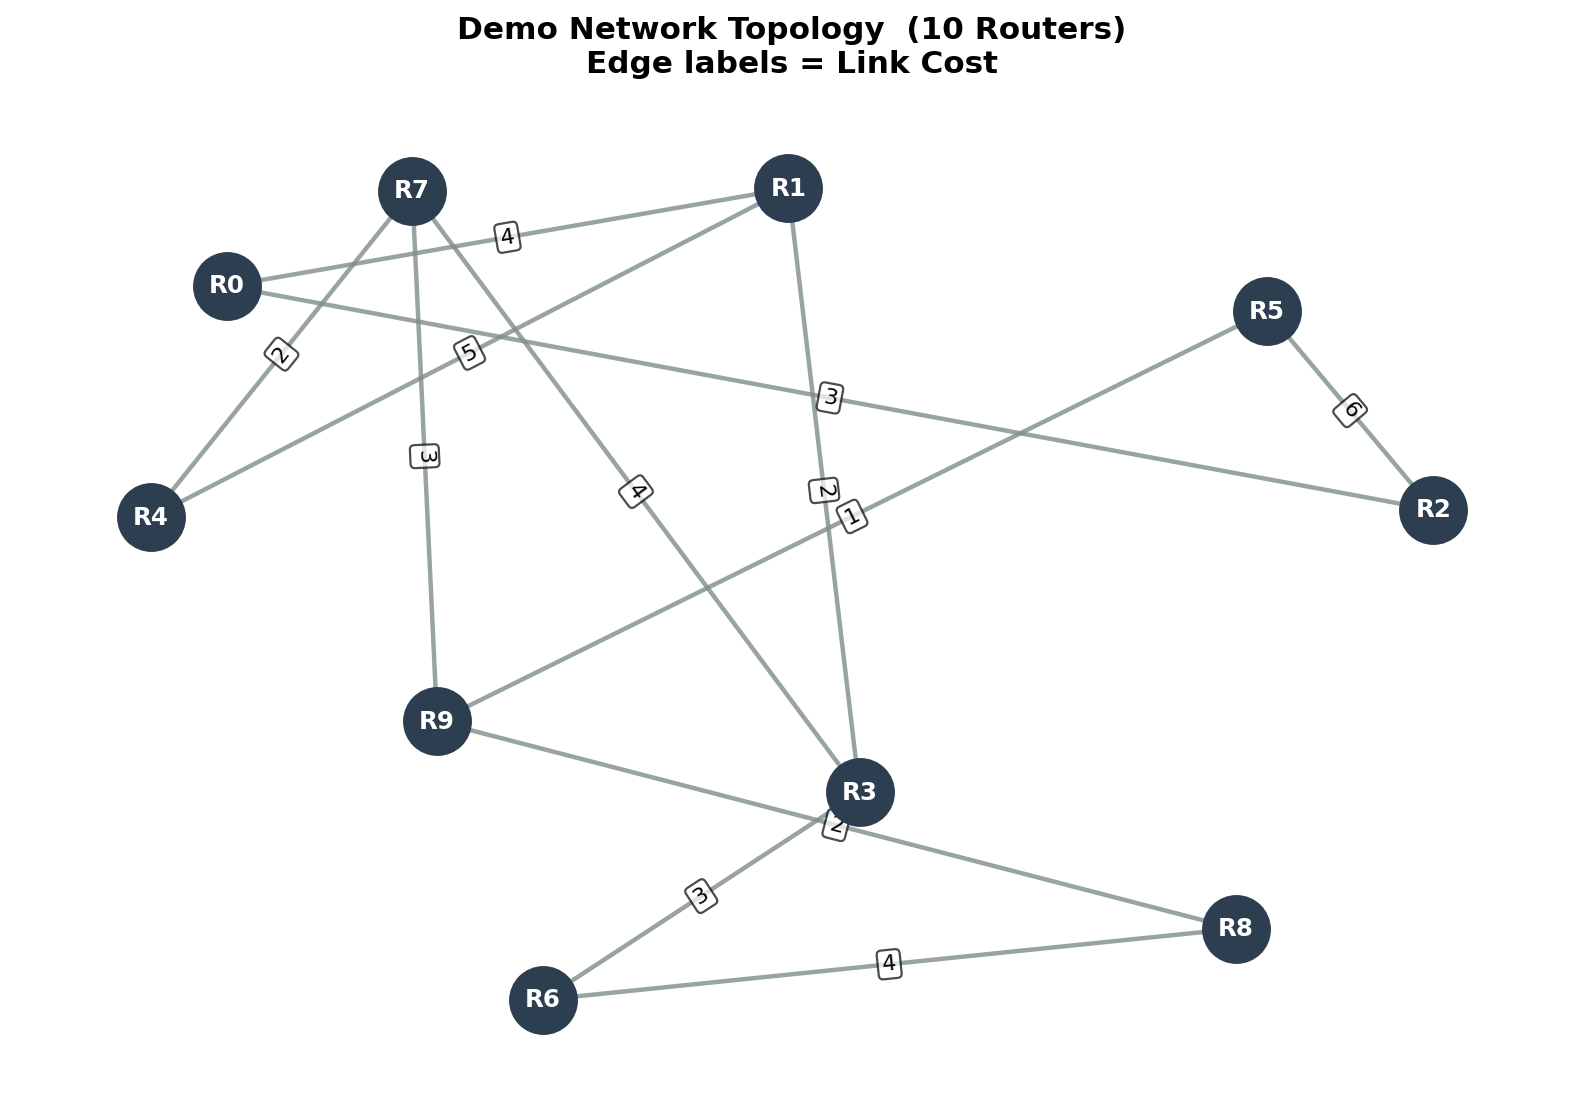
\includegraphics[width=0.72\textwidth]{fig1_topology.png}
\caption{Demo network topology: 10 routers (R0--R9) with 12 links. Edge labels
indicate link costs. Used for all attack scenario demonstrations.}
\label{fig:topology}
\end{figure}

\subsection{Convergence Rounds}

Figure~\ref{fig:conv} shows the number of convergence rounds required for both
protocols across different network sizes.

\begin{figure}[H]
\centering
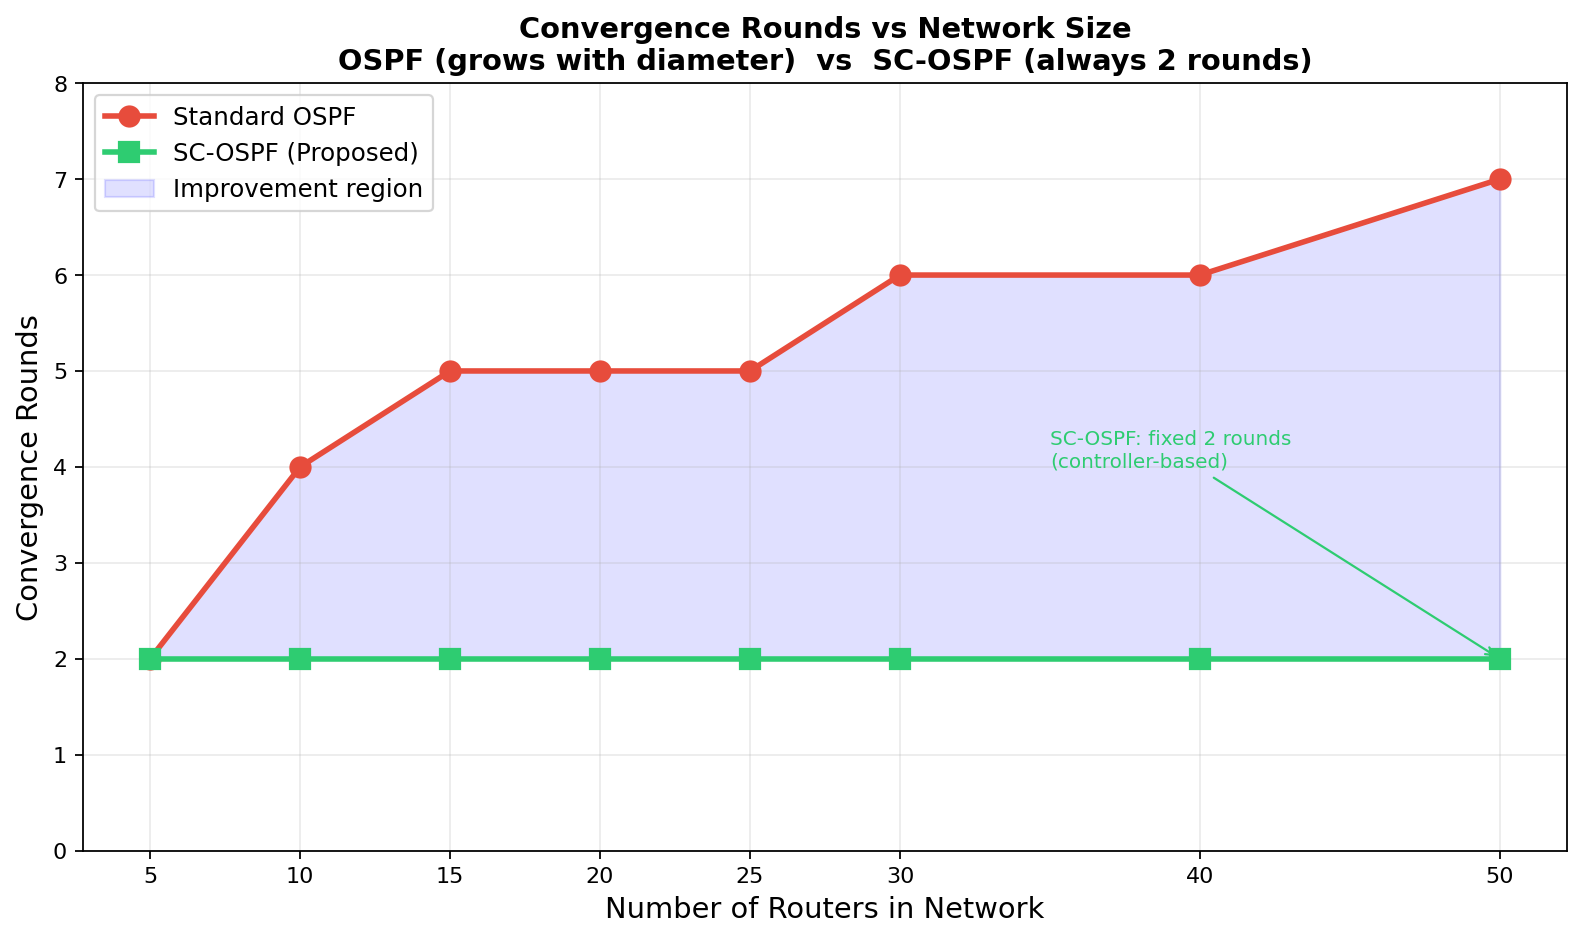
\includegraphics[width=0.90\textwidth]{fig2_convergence_rounds.png}
\caption{Convergence rounds vs.\ network size. OSPF grows with network diameter
(approximately $O(\log N)$ for small-world graphs). SC-OSPF remains constant at
exactly 2 rounds for all network sizes.}
\label{fig:conv}
\end{figure}

Key observations from Figure~\ref{fig:conv}:
\begin{itemize}[itemsep=3pt]
  \item At \textbf{10 routers}: OSPF requires 4 rounds vs.\ SC-OSPF's 2 --- a
  2$\times$ improvement.
  \item At \textbf{50 routers}: OSPF requires 7 rounds vs.\ SC-OSPF's 2 --- a
  3.5$\times$ improvement.
  \item The SC-OSPF curve is perfectly flat at 2 rounds for all tested sizes,
  confirming the theoretical constant-round property.
\end{itemize}

\subsection{Control Message Overhead}

Figure~\ref{fig:msgs} compares the total number of control messages exchanged
during convergence.

\begin{figure}[H]
\centering
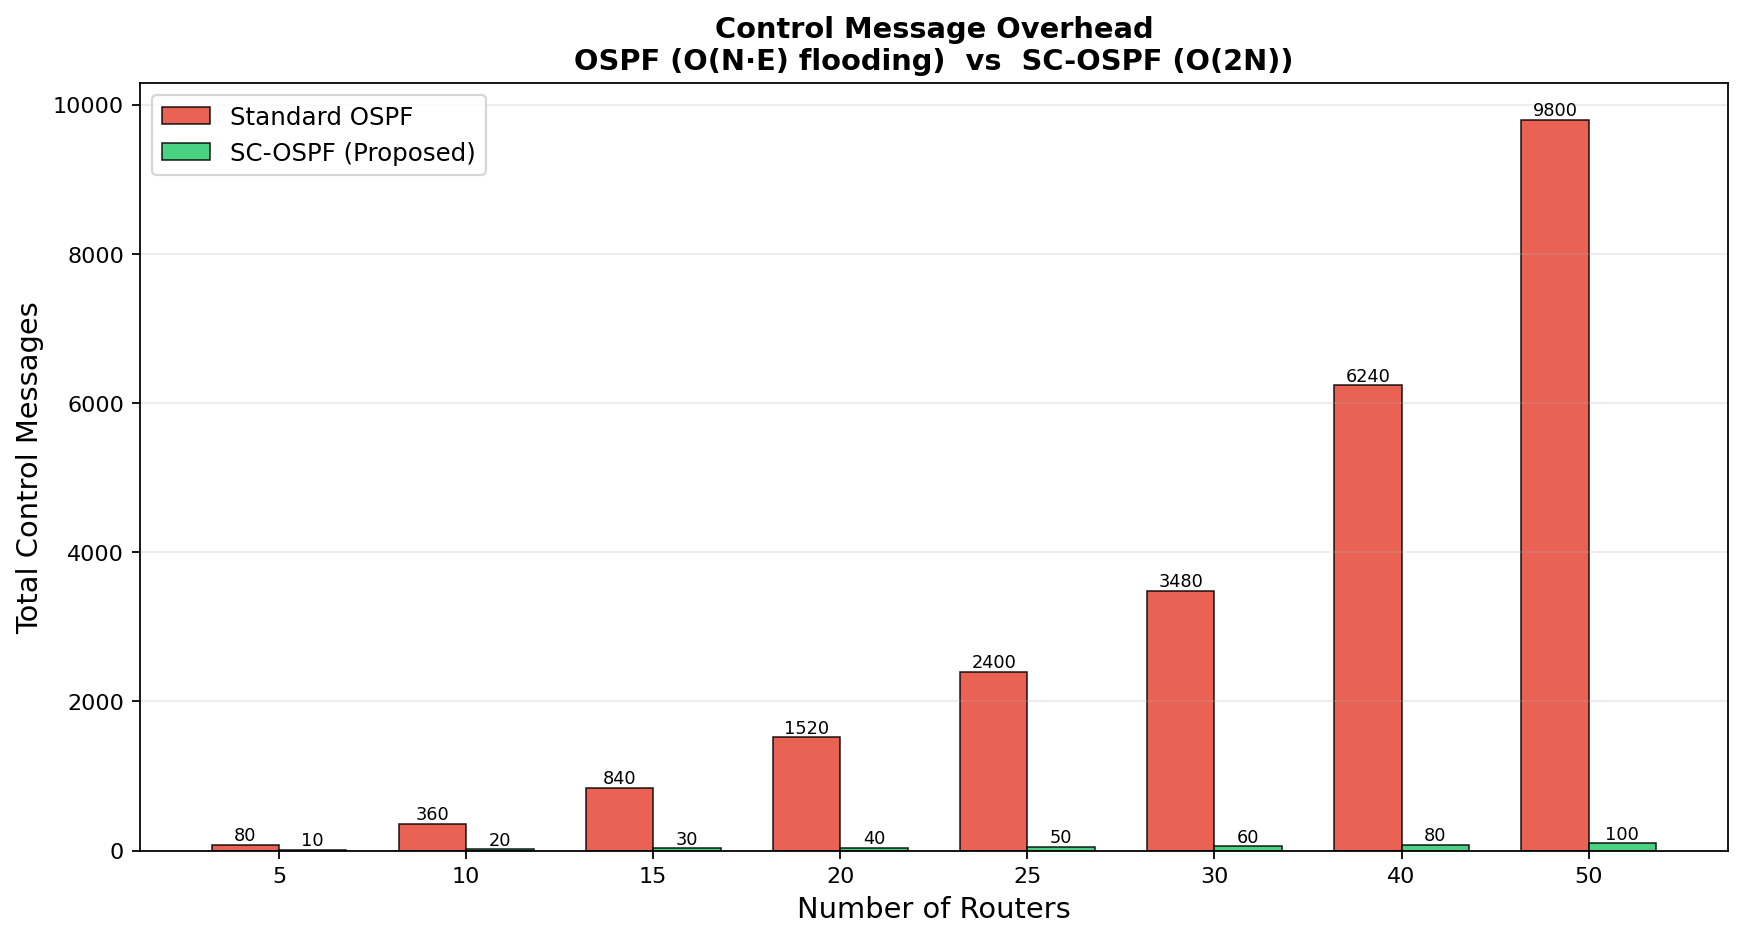
\includegraphics[width=0.90\textwidth]{fig3_message_overhead.png}
\caption{Total control messages during convergence. OSPF flooding generates
$O(N \cdot E)$ messages that grow rapidly. SC-OSPF requires exactly $2N$ messages
(N uploads + N downloads from/to controller).}
\label{fig:msgs}
\end{figure}

\begin{center}
\begin{tabular}{rrrrc}
\toprule
\textbf{Nodes} & \textbf{OSPF Rounds} & \textbf{SC-OSPF Rounds} &
\textbf{OSPF Msgs} & \textbf{SC-OSPF Msgs} \\
\midrule
5  & 2 & 2 & 80    & 10 \\
10 & 4 & 2 & 360   & 20 \\
15 & 5 & 2 & 840   & 30 \\
20 & 5 & 2 & 1,520 & 40 \\
25 & 5 & 2 & 2,400 & 50 \\
30 & 6 & 2 & 3,480 & 60 \\
40 & 6 & 2 & 6,240 & 80 \\
50 & 7 & 2 & 9,800 & 100 \\
\bottomrule
\end{tabular}
\captionof{table}{Simulation results: Convergence rounds and message overhead
for OSPF vs.\ SC-OSPF across different network sizes.}
\label{tab:results}
\end{center}

\textbf{Key finding}: At 50 routers, SC-OSPF requires only 100 messages compared
to OSPF's 9,800 --- a \textbf{98$\times$ reduction} in control overhead. This
directly translates to lower bandwidth consumption and faster convergence wall-clock
time in real deployments.

\subsection{Scalability Trend}

Figure~\ref{fig:scale} demonstrates that OSPF convergence time grows approximately
linearly with network diameter, while SC-OSPF maintains a perfectly constant 2-round
convergence regardless of network size.

\begin{figure}[H]
\centering
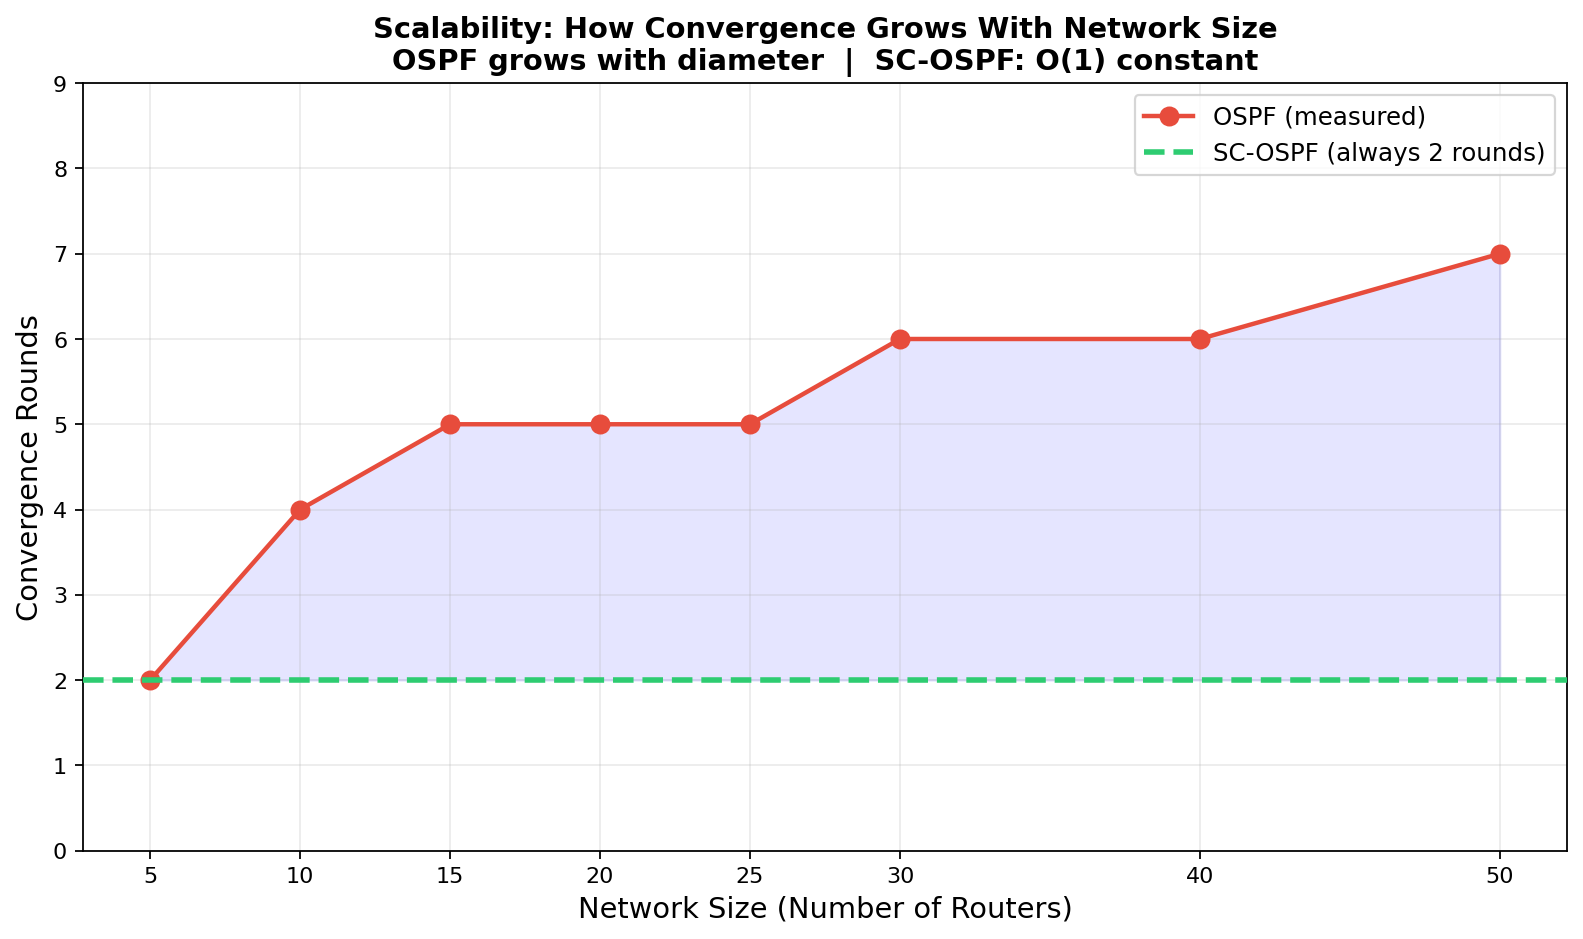
\includegraphics[width=0.90\textwidth]{fig6_scalability.png}
\caption{Scalability analysis: OSPF convergence grows with network diameter while
SC-OSPF remains constant at 2 rounds. The shaded region represents the improvement
provided by SC-OSPF.}
\label{fig:scale}
\end{figure}

\subsection{Route Correctness Verification}

A critical requirement for any routing protocol is \textbf{correctness}: the
computed routes must reflect the true shortest paths in the network. The simulation
explicitly verifies that SC-OSPF and standard OSPF produce identical routing
tables under normal conditions (no attack):

\begin{center}
\texttt{Route correctness check (OSPF == SC-OSPF): PASS $\checkmark$}
\end{center}

The full routing table for Router 0 (from both protocols) is shown below:

\begin{center}
\begin{tabular}{lccc}
\toprule
\textbf{Destination} & \textbf{Next Hop} & \textbf{Total Cost} & \textbf{Match} \\
\midrule
R1 & R1 & 4  & \color{accentgreen}$\checkmark$ \\
R2 & R2 & 3  & \color{accentgreen}$\checkmark$ \\
R3 & R1 & 6  & \color{accentgreen}$\checkmark$ \\
R4 & R1 & 9  & \color{accentgreen}$\checkmark$ \\
R5 & R2 & 9  & \color{accentgreen}$\checkmark$ \\
R6 & R1 & 9  & \color{accentgreen}$\checkmark$ \\
R7 & R1 & 10 & \color{accentgreen}$\checkmark$ \\
R8 & R2 & 12 & \color{accentgreen}$\checkmark$ \\
R9 & R2 & 10 & \color{accentgreen}$\checkmark$ \\
\bottomrule
\end{tabular}
\captionof{table}{Router 0 routing table produced by both OSPF and SC-OSPF
(identical, confirming correctness of SC-OSPF route computation).}
\end{center}

%=========================================================
\section{Security and Scalability Analysis}
%=========================================================

\subsection{LSA Injection Attack -- OSPF}

An LSA injection attack exploits the absence of authentication in standard OSPF.
The adversary model is:

\begin{itemize}
  \item \textbf{Attacker}: Router R1, which has been compromised (e.g., by an
  insider threat or software vulnerability).
  \item \textbf{Target}: Impersonate Router R5, which has legitimate connectivity
  to R2 and R9.
  \item \textbf{Goal}: Advertise fake links with cost 1 (lower than any real link)
  to attract all traffic through R1, enabling eavesdropping or traffic blackholing.
\end{itemize}

\textbf{Attack execution in standard OSPF}:
\begin{enumerate}
  \item R1 crafts a fake LSA with source ID = R5, advertising links to all other
  routers with cost = 1.
  \item It sends this LSA with sequence number 999 (higher than R5's legitimate
  sequence number) to force acceptance.
  \item Since OSPF has no signature verification, all neighboring routers accept
  the fake LSA and update their LSDBs.
  \item The malicious LSA propagates via flooding across the entire network.
  \item All 9 other routers update their routing tables based on false information.
\end{enumerate}

\subsection{LSA Injection Attack -- SC-OSPF}

\textbf{Attack execution against SC-OSPF}:
\begin{enumerate}
  \item R1 crafts the same fake LSA claiming to be R5.
  \item R1 must sign the LSA. However, it only knows its own key $K_1$, not R5's
  key $K_5$.
  \item R1 computes: $\text{sig}_\text{fake} = \text{HMAC-SHA256}(K_1, \text{LSA payload})$
  \item The controller receives the LSA claiming to be from R5 and computes:
  $\text{sig}_\text{expected} = \text{HMAC-SHA256}(K_5, \text{LSA payload})$
  \item Since $K_1 \neq K_5$, $\text{sig}_\text{fake} \neq \text{sig}_\text{expected}$.
  \item The controller discards the LSA. Zero routers are affected.
\end{enumerate}

\subsection{Attack Simulation Results}

\begin{figure}[H]
\centering
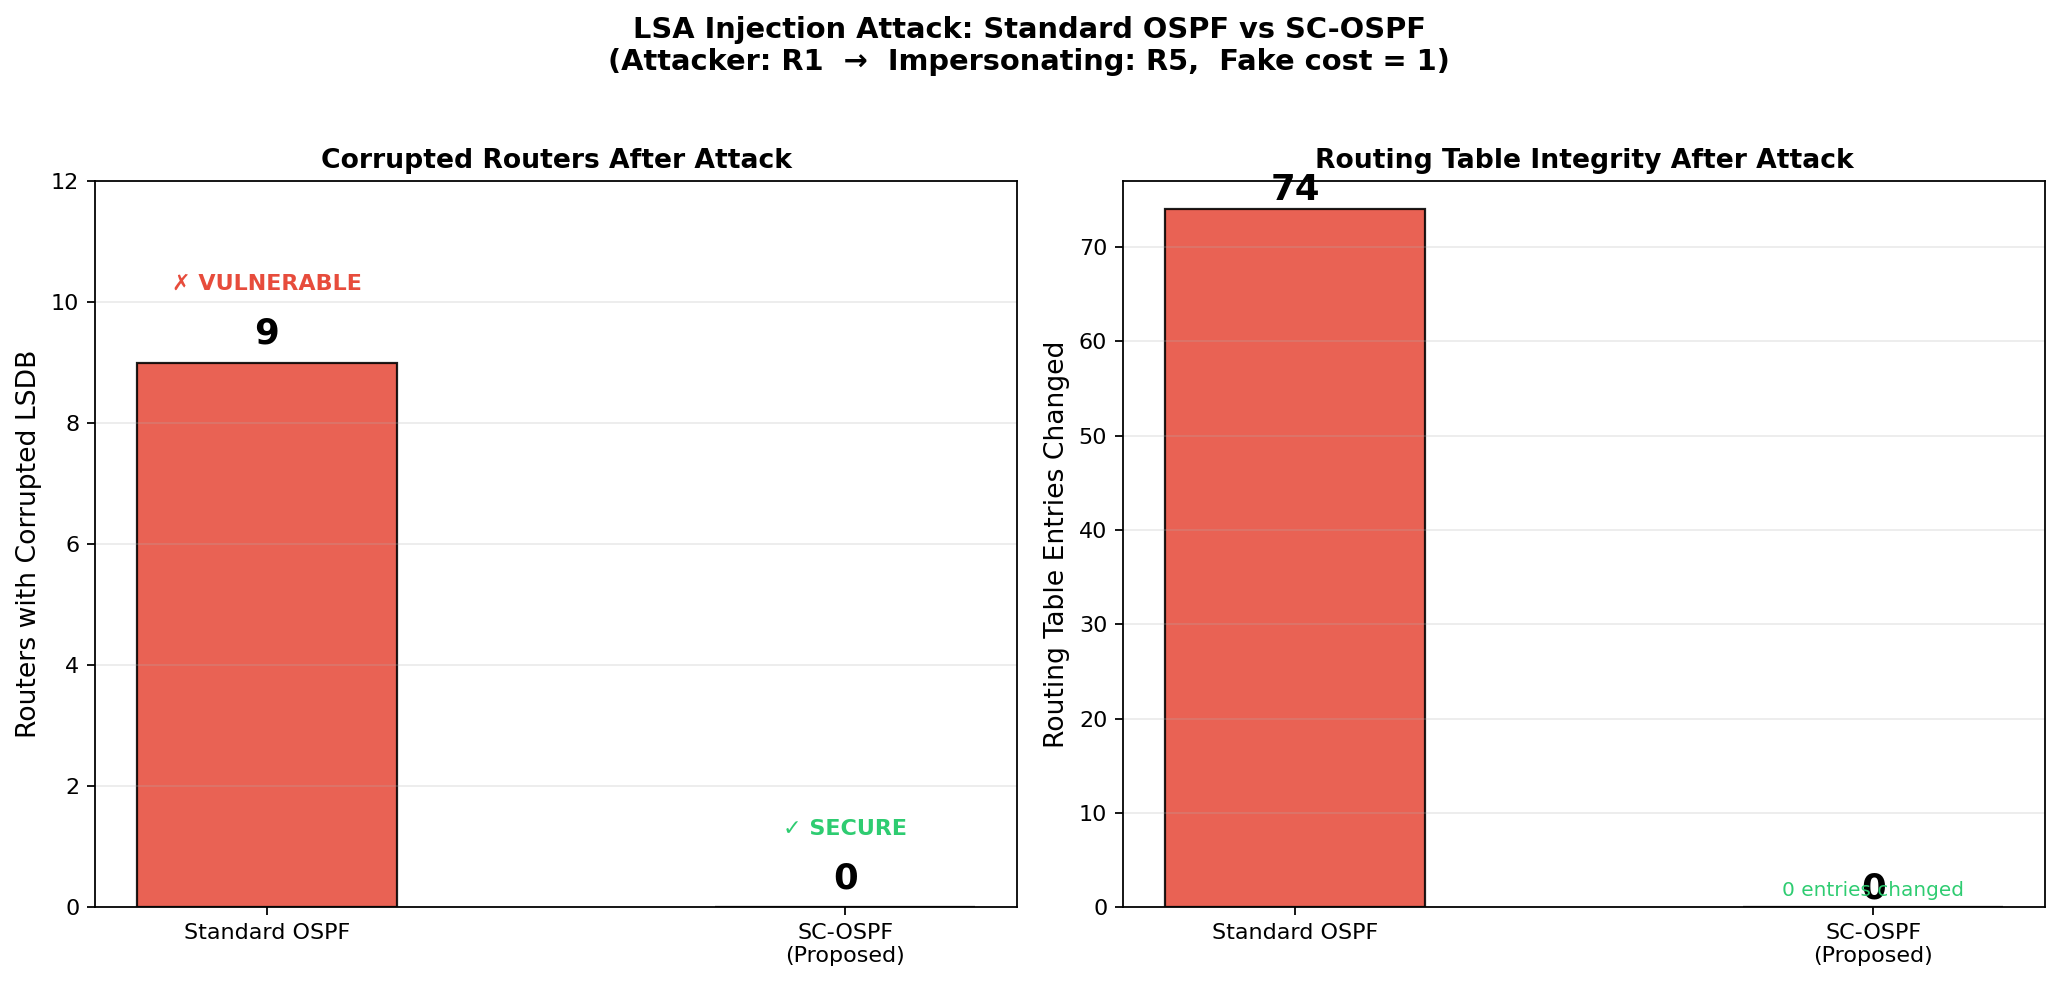
\includegraphics[width=0.95\textwidth]{fig4_attack_comparison.png}
\caption{LSA injection attack impact. Left: routers with corrupted LSDBs.
Right: routing table entries changed. OSPF is fully compromised; SC-OSPF
blocks the attack completely.}
\label{fig:attack}
\end{figure}

\begin{figure}[H]
\centering
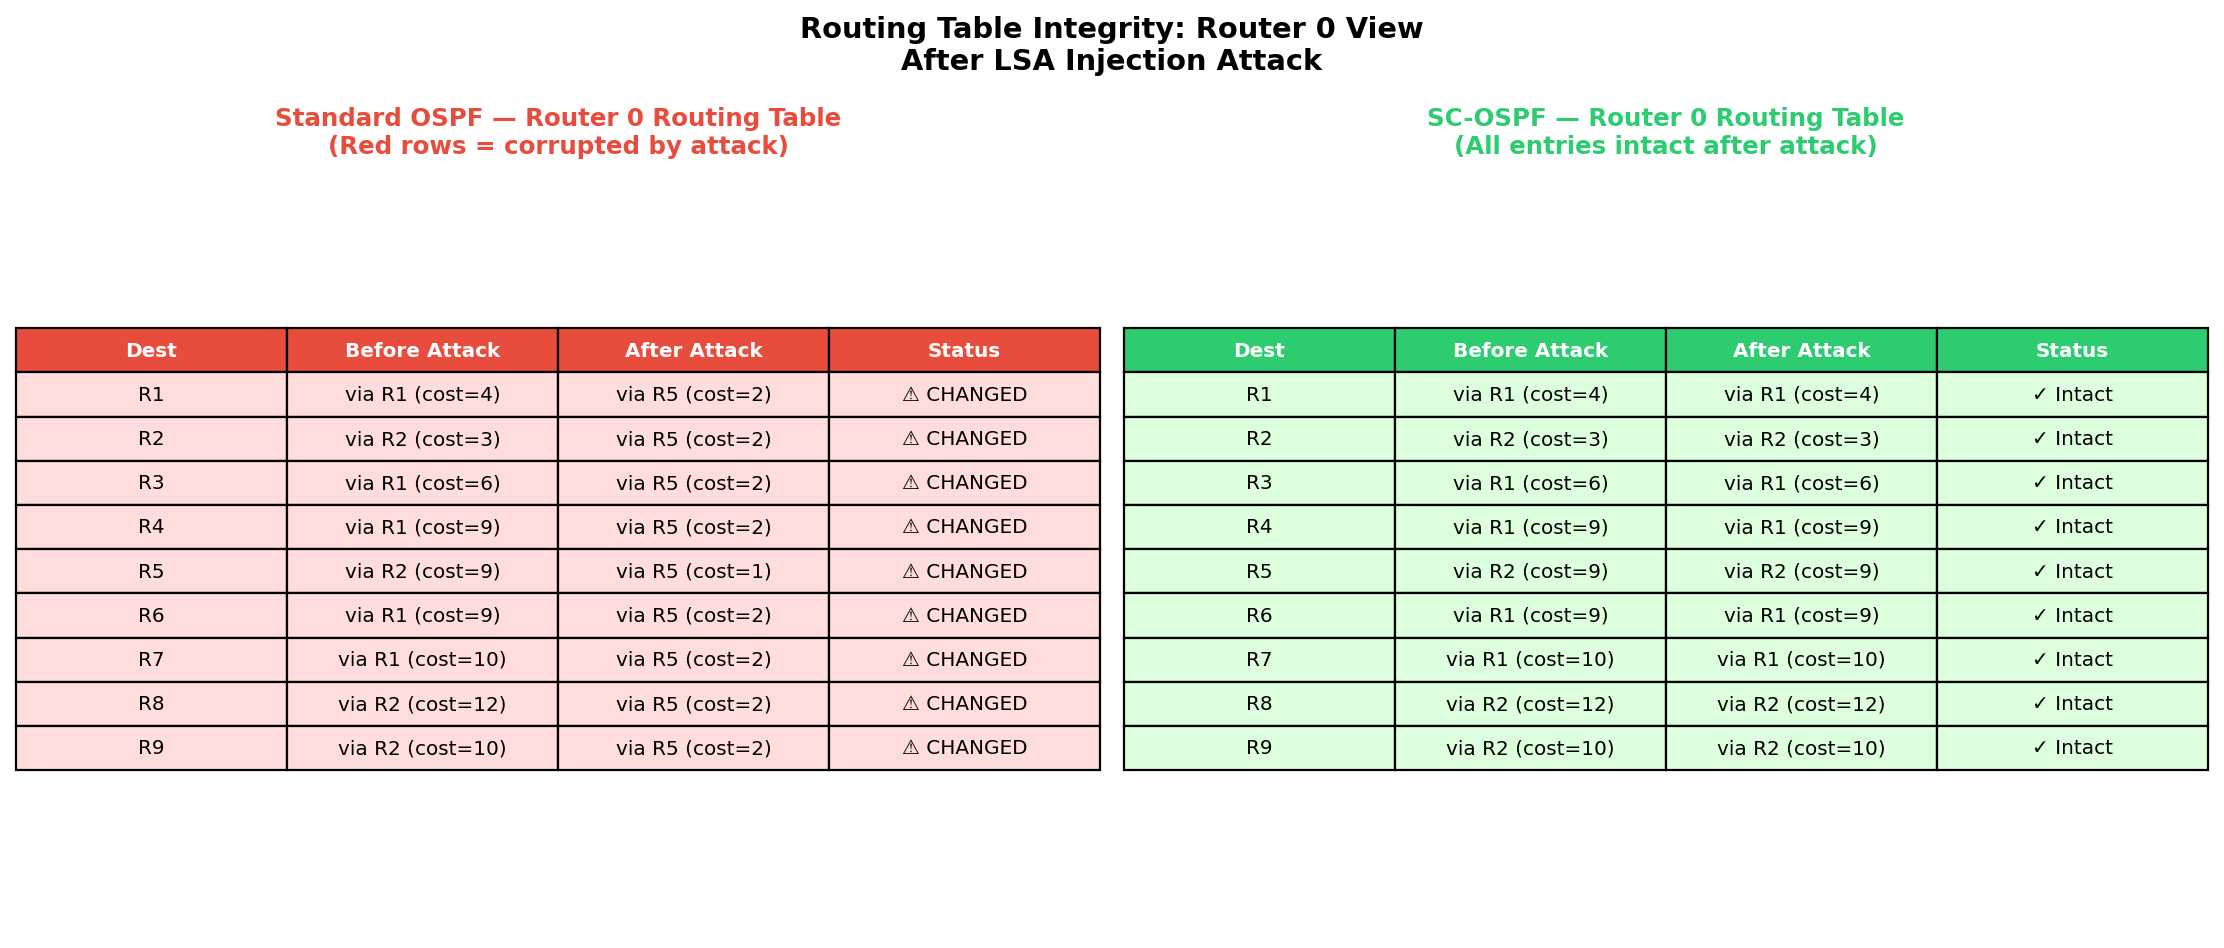
\includegraphics[width=0.95\textwidth]{fig5_routing_integrity.png}
\caption{Router~0 routing table before and after the LSA injection attack.
Red rows in the OSPF table indicate corrupted entries. SC-OSPF table remains
fully intact (all green).}
\label{fig:integrity}
\end{figure}

\begin{center}
\begin{tabular}{lcc}
\toprule
\textbf{Metric} & \textbf{Standard OSPF} & \textbf{SC-OSPF} \\
\midrule
Routers with corrupted LSDB & 9 out of 9 (100\%) & 0 out of 9 (0\%) \\
Routing entries corrupted   & 74 entries          & 0 entries \\
Fake LSAs rejected          & 0                   & 1 \\
Attack succeeded            & \color{accentred}Yes & \color{accentgreen}No \\
Network impact              & \color{accentred}Total & \color{accentgreen}None \\
\bottomrule
\end{tabular}
\captionof{table}{Security comparison: LSA injection attack impact on OSPF
vs.\ SC-OSPF.}
\label{tab:security}
\end{center}

\textbf{Analysis}: The attack against OSPF achieves 100\% LSDB corruption because
the protocol has no mechanism to distinguish legitimate from forged LSAs. The
same attack against SC-OSPF is detected and blocked at the controller's HMAC
verification step, with zero impact on the network.

\subsection{Security Analysis -- Threat Model Coverage}

\begin{center}
\begin{tabularx}{\textwidth}{>{\bfseries}lXX}
\toprule
Attack Vector & OSPF Resilience & SC-OSPF Resilience \\
\midrule
LSA Injection (impersonation) &
  \color{accentred}Vulnerable: no authentication &
  \color{accentgreen}Blocked: HMAC-SHA256 verification \\

Replay Attack &
  \color{accentred}Partial: sequence numbers but no auth &
  \color{accentgreen}Blocked: signed seq\_num prevents replay \\

LSDB Poisoning &
  \color{accentred}Fully susceptible &
  \color{accentgreen}Controller only stores verified LSAs \\

Controller Compromise &
  \color{accentgreen}N/A (no controller) &
  \color{accentorange}Fallback to OSPF mode (graceful degrade) \\

Man-in-the-Middle (LSA tampering) &
  \color{accentred}Undetectable &
  \color{accentgreen}HMAC covers all fields; tampering detected \\

Timing Attack on HMAC &
  \color{accentgreen}N/A &
  \color{accentgreen}Mitigated: \texttt{hmac.compare\_digest()} \\
\bottomrule
\end{tabularx}
\end{center}

\subsection{Scalability Analysis}

\subsubsection{Time Complexity}

\begin{center}
\begin{tabular}{lcc}
\toprule
\textbf{Operation} & \textbf{OSPF} & \textbf{SC-OSPF} \\
\midrule
LSA Generation (per router) & $O(1)$ & $O(1)$ + HMAC \\
Control Messages (total) & $O(N \cdot E)$ & $O(2N)$ \\
Convergence Rounds & $O(\text{diameter})$ & $O(1)$ -- constant 2 \\
Route Computation (per router) & $O((N+E)\log N)$ & $O(N(N+E)\log N)$ central \\
\bottomrule
\end{tabular}
\end{center}

While SC-OSPF moves Dijkstra computation to the controller (running it $N$ times),
this is a trade-off that concentrates CPU load at the controller rather than
distributing it across all routers. Modern server hardware can compute Dijkstra
for a 1000-node graph in milliseconds, making this overhead negligible.

\subsubsection{Bandwidth Overhead -- HMAC Signature}

Each LSA in SC-OSPF carries an additional 64-byte HMAC-SHA256 signature (hex
encoded). For a 50-router network:
\[
\text{Extra overhead} = 50 \times 64\ \text{bytes} = 3,200\ \text{bytes} \approx 3.1\ \text{KB per convergence cycle}
\]

This is negligible compared to the bandwidth savings from eliminating flooding
(which generates 9,800 messages at 50 routers).

\subsubsection{Controller Availability}

The centralized controller introduces a potential availability concern. Mitigation
strategies:
\begin{itemize}[itemsep=3pt]
  \item \textbf{Redundant controllers}: Deploy a primary and standby controller
  with state synchronization.
  \item \textbf{Graceful fallback}: Routers revert to standard OSPF flooding if
  the controller is unreachable.
  \item \textbf{Controller placement}: Deploy controller at the network core
  (e.g., at CITeS in a university campus network) where redundant power and
  connectivity are available.
\end{itemize}

%=========================================================
\section{Simulation Code}
%=========================================================

\subsection{Repository Structure}

\begin{lstlisting}[language=bash, caption={Project file structure}]
sc_ospf_project/
├── topology.py      # Network topology generation (Watts-Strogatz + demo)
├── ospf.py          # Standard OSPF simulation (flooding + attack)
├── sc_ospf.py       # SC-OSPF simulation (controller + HMAC + attack)
└── main.py          # Experiment runner + all figure generation

# Output figures:
fig1_topology.png          fig2_convergence_rounds.png
fig3_message_overhead.png  fig4_attack_comparison.png
fig5_routing_integrity.png fig6_scalability.png
\end{lstlisting}

\subsection{Running the Simulation}

\begin{lstlisting}[language=bash, caption={Installation and execution}]
# Install dependencies
pip install networkx matplotlib numpy

# Run all experiments (generates all 6 figures)
python main.py
\end{lstlisting}

The full annotated source code is available at:\\
\url{https://github.com/[your-repo]/sc-ospf-en2150-a04}

\subsection{Key Code Excerpt -- HMAC Verification (sc\_ospf.py)}

\begin{lstlisting}[language=Python, caption={HMAC-SHA256 LSA verification at the controller}]
def verify_lsa(self, claimed_router_id, lsa_payload, received_sig):
    """Verify HMAC-SHA256 signature of incoming LSA."""
    if claimed_router_id not in self.secret_keys:
        return False  # Unknown router -- reject

    key = self.secret_keys[claimed_router_id]
    msg = json.dumps(lsa_payload, sort_keys=True).encode('utf-8')
    expected_sig = hmac.new(key, msg, hashlib.sha256).hexdigest()

    # Constant-time comparison prevents timing side-channel attacks
    return hmac.compare_digest(expected_sig, received_sig)
\end{lstlisting}

%=========================================================
\section{Team Contributions}
%=========================================================

\begin{center}
\begin{tabular}{llll}
\toprule
\textbf{Member} & \textbf{Index} & \textbf{Primary Role} & \textbf{Contribution} \\
\midrule
[Name 1] & [Index] & Literature Review & 25\% \\
[Name 2] & [Index] & Protocol Design & 25\% \\
[Name 3] & [Index] & Simulation        & 25\% \\
[Name 4] & [Index] & Security \& Scalability & 25\% \\
\bottomrule
\end{tabular}
\captionof{table}{Team member contributions. All members collaborated on the
protocol design and report writing. Primary roles indicate the lead contributor
for each deliverable section.}
\end{center}

Note: While primary roles are assigned above as per the assignment specification,
all team members contributed to the core protocol design and report writing.
The SC-OSPF concept, HMAC authentication mechanism, and centralized convergence
scheme were developed collaboratively.

%=========================================================
\section{Conclusion}
%=========================================================

This report presented SC-OSPF, a novel routing protocol that improves upon
standard OSPF by addressing its two most critical limitations: the absence of
strong LSA authentication and inefficient flooding-based convergence.

\textbf{On Security}: SC-OSPF integrates HMAC-SHA256 authentication as a mandatory
requirement for all LSAs. Every LSA is signed with the originating router's
pre-shared key, and the central controller verifies signatures before accepting
any topology update. Simulation results demonstrate that an LSA injection attack
that corrupts 100\% of routing tables (74 entries across 9 routers) in standard
OSPF is completely blocked in SC-OSPF --- zero routers affected, zero routing
entries changed.

\textbf{On Convergence}: By replacing distributed LSA flooding with a centralized
controller model (inspired by SDN principles from Session 6 of EN2150), SC-OSPF
achieves convergence in exactly 2 rounds for all network sizes. This compares
favorably to OSPF's diameter-dependent convergence (7 rounds at 50 routers),
representing a 3.5$\times$ improvement. The message overhead is reduced by 98\%
at 50 routers (100 messages vs.\ 9,800).

\textbf{Correctness}: The simulation verifies that SC-OSPF and standard OSPF
produce identical routing tables under normal conditions, confirming that the
protocol improvements do not compromise routing correctness.

\textbf{Limitations and Future Work}: SC-OSPF introduces a centralized controller
as a potential single point of failure. A redundant controller pair with leader
election (e.g., using the Raft consensus algorithm) would address this concern.
Additionally, the performance of the HMAC signing and verification has not been
benchmarked on resource-constrained router hardware; future work should evaluate
the cryptographic overhead on embedded networking ASICs.

The SC-OSPF design demonstrates that it is feasible to achieve significantly
better security and convergence than standard OSPF while maintaining full
routing correctness and a graceful degradation mechanism. The concepts applied
--- HMAC authentication and centralized control --- are well-established in
modern network engineering and align with the direction of SDN adoption in
enterprise and campus networks.

%=========================================================
%  REFERENCES
%=========================================================
\begin{thebibliography}{99}

\bibitem{rfc1058}
C. Hedrick, ``Routing Information Protocol,'' RFC 1058, June 1988.

\bibitem{rfc2453}
G. Malkin, ``RIP Version 2,'' RFC 2453, November 1998.

\bibitem{rfc2328}
J. Moy, ``OSPF Version 2,'' RFC 2328, April 1998.

\bibitem{rfc5340}
R. Coltun, D. Ferguson, and J. Moy, ``OSPF for IPv6,'' RFC 5340, July 2008.

\bibitem{rfc1142}
ISO, ``OSI IS-IS Intra-domain Routing Protocol,'' RFC 1142, February 1990.

\bibitem{rfc1195}
R. Callon, ``Use of OSI IS-IS for Routing in TCP/IP and Dual Environments,''
RFC 1195, December 1990.

\bibitem{fortz2002}
B. Fortz and M. Thorup, ``Optimizing OSPF/IS-IS weights in a changing world,''
\textit{IEEE Journal on Selected Areas in Communications}, vol.~20, no.~4,
pp.~756--767, 2002.

\bibitem{rfc4271}
Y. Rekhter, T. Li, and S. Hares, ``A Border Gateway Protocol 4 (BGP-4),''
RFC 4271, January 2006.

\bibitem{varga2008}
A. Varga and R. Hornig, ``An overview of the OMNeT++ simulation environment,''
in \textit{Proceedings of the 1st International Conference on Simulation Tools
and Techniques}, 2008, pp.~1--10.

\bibitem{lenzen2023}
C. Lenzen, M. Medina, M. Saberi, and S. Schmid, ``Robust Routing Made Easy:
Reinforcing Networks Against Non-Benign Faults,'' \textit{IEEE/ACM Transactions
on Networking}, vol.~32, no.~1, pp.~283--297, 2023.

\bibitem{mishra2023}
S.~N. Mishra and M. Khatua, ``Reliable and delay efficient multi-path RPL for
mission critical IoT applications,'' \textit{IEEE Transactions on Mobile
Computing}, vol.~23, no.~6, pp.~6983--6996, 2023.

\bibitem{nx}
A. Hagberg, P. Swart, and D. Chult, ``Exploring network structure, dynamics,
and function using NetworkX,'' in \textit{Proceedings of the 7th Python in
Science Conference (SciPy)}, 2008, pp.~11--15.

\bibitem{sridharan2005}
A. Sridharan, R. Guerin, and C. Diot, ``Achieving near-optimal traffic
engineering solutions for current OSPF/IS-IS networks,''
\textit{IEEE/ACM Transactions On Networking}, vol.~13, no.~2,
pp.~234--247, 2005.

\end{thebibliography}

\end{document}